% !TEX TS-program = pdflatex
% !TEX encoding = UTF-8 Unicode

% This is a simple template for a LaTeX document using the "article" class.
% See "book", "report", "letter" for other types of document.

\documentclass[11pt]{article} % use larger type; default would be 10pt

\usepackage[utf8]{inputenc} % set input encoding (not needed with XeLaTeX)

%%% Examples of Article customizations
% These packages are optional, depending whether you want the features they provide.
% See the LaTeX Companion or other references for full information.

%%% PAGE DIMENSIONS
\usepackage{geometry} % to change the page dimensions
\geometry{a4paper} % or letterpaper (US) or a5paper or....
% \geometry{margin=2in} % for example, change the margins to 2 inches all round
% \geometry{landscape} % set up the page for landscape
%   read geometry.pdf for detailed page layout information

\usepackage{graphicx} % support the \includegraphics command and options
\usepackage{alltt}
\usepackage{wrapfig}
% \usepackage[parfill]{parskip} % Activate to begin paragraphs with an empty line rather than an indent

%%% PACKAGES
\usepackage{booktabs} % for much better looking tables
\usepackage{array} % for better arrays (eg matrices) in maths
\usepackage{amssymb}
\usepackage{paralist} % very flexible & customisable lists (eg. enumerate/itemize, etc.)
\usepackage{verbatim} % adds environment for commenting out blocks of text & for better verbatim
\usepackage{subfig} % make it possible to include more than one captioned figure/table in a single float
% These packages are all incorporated in the memoir class to one degree or another...

%%% HEADERS & FOOTERS
\usepackage{fancyhdr} % This should be set AFTER setting up the page geometry
\pagestyle{fancy} % options: empty , plain , fancy
\renewcommand{\headrulewidth}{0pt} % customise the layout...
\lhead{}\chead{}\rhead{}
\lfoot{}\cfoot{\thepage}\rfoot{}

%%% SECTION TITLE APPEARANCE
\usepackage{sectsty}
\allsectionsfont{\sffamily\mdseries\upshape} % (See the fntguide.pdf for font help)
% (This matches ConTeXt defaults)

%%% ToC (table of contents) APPEARANCE
\usepackage[nottoc,notlof,notlot]{tocbibind} % Put the bibliography in the ToC
\usepackage[titles,subfigure]{tocloft} % Alter the style of the Table of Contents
\renewcommand{\cftsecfont}{\rmfamily\mdseries\upshape}
\renewcommand{\cftsecpagefont}{\rmfamily\mdseries\upshape} % No bold!

%%% END Article customizations

%%% The "real" document content comes below...

\title{Numerical Analysis Project 1}
\author{Margaret Dorsey}
%\date{} % Activate to display a given date or no date (if empty),
         % otherwise the current date is printed 

\newenvironment{claim}[1]{\par\noindent\underline{Claim:}\space#1}{}
\newenvironment{proof}[1]{\par\noindent\underline{Proof:}\space#1}{\hfill $\blacksquare$}

\begin{document}
\maketitle

\section*{Graphical Illustration of the Function}

\section*{Positive Solutions of X}


\begin{claim}
There is exactly one positive solution for $x$.
\end{claim}
\begin{proof}

%% show f(0) < 0
We first note $f(0) < 0$ for all values of $k$ ,$\eta$, $\xi$ - when $x = 0$, the rest of the function $f(x)$ disappears, leaving us with $f(0) = -\xi$, a negative value, because $\xi$ represents ligand concentration, a physical quantity, and thus must be positive (because $0$ is a trivial case and negative values are non-physical).
%% find and demonstrate an x such that f(x) > 0, x is large
\par Additionally, for $x = \xi$, $f(x) > 0$, because $f(x) = \xi - \xi + \sum_{j=1}^{M} \frac{k_j \eta_j}{1+k_j\eta}$ in this case, where all of the sum terms are non-negative, and at least one is non-zero (otherwise it is modelling a trivial case where there is no amount of any binding molecules).
%% thus there is a root due to intermediate value theorem, f is continuous
\par Thus, by the intermediate value theorem, we know that $f$ has at least one positive root between $0$ and $\xi$. Calculating the derivative with respect to $x$ of $f$, we get
	$$f'(x) = 1 + \sum_{j=1}^{M} = \frac{k_j \eta_j}{(1+k_jx)^2}$$
%% show function is strictly increasing for positive x using the derivative
which by reasoning analogous to the above argument, is always positive for positive $x$. Thus $f(x)$ is strictly increasing for positive $x$, and due to Rolle's theorem, we know that $f(x)$ restricted to positive $x$ has at most one root, which completes the proof.
%%a strictly increasing function has at most one root, due to Rolle's Theorem
%% done

\end{proof}

\section*{Fixed Point Iteration}

\subsection*{Finding $g(x)$}

\subsubsection*{Case Testing}
%%show it works for case 1, not for case 2
\begin{alltt}
Enter the initial guess for the first test: 1 

--------------------------
 Fixed Point Iteration
 -----------------------


i: 0	x: 1.000000000	value: 2.500000000
i: 1	x: 2.500000000	value: 2.285714286
i: 2	x: 2.285714286	value: 2.304347826
i: 3	x: 2.304347826	value: 2.302631579
i: 4	x: 2.302631579	value: 2.302788845
i: 5	x: 2.302788845	value: 2.302774427
i: 6	x: 2.302774427	value: 2.302775749
i: 7	x: 2.302775749	value: 2.302775628
i: 8	x: 2.302775628	value: 2.302775639
i: 9	x: 2.302775639	value: 2.302775638

Enter the initial guess for the second test:  1

--------------------------
 Fixed Point Iteration
 -----------------------


i: 0	x: 1.000000000	value: 0.500000000
i: 1	x: 0.500000000	value: 1.333333333
i: 2	x: 1.333333333	value: 0.142857143
i: 3	x: 0.142857143	value: 2.375000000
i: 4	x: 2.375000000	value: -0.518518519
i: 5	x: -0.518518519	value: 8.384615385
i: 6	x: 8.384615385	value: -1.467213115
\vdots
i: 54	x: -3.791287852	value: -3.791287845
i: 55	x: -3.791287845	value: -3.791287849
i: 56	x: -3.791287849	value: -3.791287846
i: 57	x: -3.791287846	value: -3.791287848
i: 58	x: -3.791287848	value: -3.791287847
\end{alltt}
%% discuss the problem here
\par Even though the proposed $g(x)$ converged in both cases, it converged to the negative root in the second case, even though the initial guess
was closer to the positive root (which is approximately $0.79$). This is because surrounding the positive root, the absolute value of $g'(x)$ is greater than $1$ in the second case, meaning that, by the contration theorem, it cannot converge to that root (because as it approaches it, the sequence will begin to diverge rather than converge).
%% use contraction theorem

\subsubsection*{Choosing $\alpha$}

%% find an alpha that works 

\begin{claim}
If $\alpha  = \sum_{j=1}^M k_jn_j$, the FPI always converges.
\end{claim}
\begin{proof}
\end{proof}


\section*{Newton's Method}

\subsection*{Test One Output}
%initial guess 1.6, what do you dislike about results
\begin{alltt}
Enter the intial guess: 1.6

--------------------------
 Newton
 -----------------------


i: 0	x: -1.124105012	value: 88.452818065
i: 1	x: -1.260131012	value: 46.182036757
i: 2	x: -1.570535828	value: 24.956847208
i: 3	x: -2.357298970	value: 14.010274589
i: 4	x: -4.536830098	value: 7.290560454
i: 5	x: -8.588461093	value: 1.729329152
i: 6	x: -10.061914568	value: 0.041604994
i: 7	x: -10.099003088	value: 0.000018410
i: 8	x: -10.099019514	value: 0.000000000

\end{alltt}

\subsection*{Test Two Output}
\subsubsection*{Output}
%initial guess 1.4999, discuss results
\begin{alltt}
Enter the intial guess: 1.4999

--------------------------
 Newton
 -----------------------


i: 0	x: -0.999876924	value: -81242.749956933
i: 1	x: -0.999753861	value: -40619.374953876
i: 2	x: -0.999507770	value: -20307.687427792
i: 3	x: -0.999015733	value: -10151.843615770
i: 4	x: -0.998032241	value: -5073.921612311
i: 5	x: -0.996067582	value: -2534.960417718
i: 6	x: -0.992147546	value: -1265.479442812
i: 7	x: -0.984344518	value: -630.738232506
i: 8	x: -0.968885874	value: -313.366310246
i: 9	x: -0.938552168	value: -154.678222468
i: 10	x: -0.880170250	value: -75.331900493
i: 11	x: -0.772155001	value: -35.661641481
i: 12	x: -0.587979613	value: -15.858623262
i: 13	x: -0.323256320	value: -6.099899665
i: 14	x: -0.056125978	value: -1.650760190
i: 15	x: 0.078909646	value: -0.189707093
i: 16	x: 0.098689910	value: -0.003059278
i: 17	x: 0.099019425	value: -0.000000818
i: 18	x: 0.099019514	value: -0.000000000

\end{alltt}


\subsection*{Test Three Output}
% guess 1.5, discuss results, they should be horrible
\begin{alltt}

Enter the intial guess: 1.5

--------------------------
 Newton
 -----------------------


i: 0	x: -1.000000000	value: -inf
i: 1	x: -nan	value: -nan

\end{alltt}


\subsection*{Test Four Output}
% guess 1.0, should be nice
\begin{alltt}
Enter the intial guess: 1.0

--------------------------
 Newton
 -----------------------


i: 0	x: -0.428571429	value: -8.928571429
i: 1	x: -0.146245059	value: -2.859208022
i: 2	x: 0.048003192	value: -0.493952479
i: 3	x: 0.096885702	value: -0.019834462
i: 4	x: 0.099015816	value: -0.000034315
i: 5	x: 0.099019514	value: -0.000000000

\end{alltt}

\subsection*{Analysis}
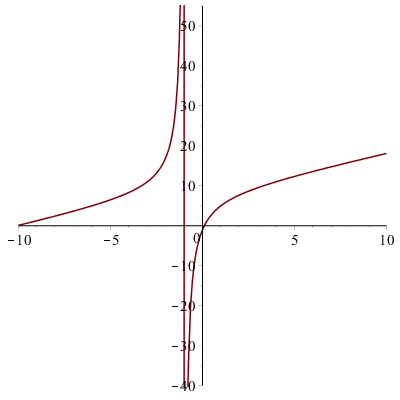
\includegraphics[scale=.5]{plots/newtongraph1.png}


\par For an initial guess of 1.6, the method successfully converged, however unfortunately it was to the negative root. For 1.499, the method converged (somewhat slowly, for newton's method) to the correct root, however 1.5 leads to division by zero. Examining the graph of f(x), the cause of this behavior becomes fairly apparent - as the positive side of the graph flattens and the slope of the tangent line approaches $0$, Newton's method tends to send $x_{n+1}$ through and across the singularity at $x = -1$, into the negative values of $x$. For $x$ before this jump across the singularity of $f(x)$, such as $1.4999$, the method, although displaced into negative $x$, can self-correct back towards the positive root. As the slope of $f(x)$ gets more and more positive approaching the positive root, Newton's method manages to converge more and more efficiently, as evidenced by the results of initial guess $1.0$.

\newpage
\section*{Algorithm Comparison}

\subsection*{Output Evaluation}
\begin{alltt}
--------------------------
 Bisection
 -----------------------


i: 0	a: 2.000000000	b: 4.000000000	value: -2.343589744 
i: 1	a: 3.000000000	b: 4.000000000	value: -0.981203008 
i: 2	a: 3.500000000	b: 4.000000000	value: -0.364898990 
i: 3	a: 3.750000000	b: 4.000000000	value: -0.066547000 
i: 4	a: 3.750000000	b: 3.875000000	value: 0.080649333 
i: 5	a: 3.750000000	b: 3.812500000	value: 0.007204681 
i: 6	a: 3.781250000	b: 3.812500000	value: -0.029631976 
i: 7	a: 3.796875000	b: 3.812500000	value: -0.011203954 
\vdots
i: 26	a: 3.806382805	b: 3.806382835	value: -0.000000012 
i: 27	a: 3.806382805	b: 3.806382820	value: 0.000000005 
i: 28	a: 3.806382813	b: 3.806382820	value: -0.000000003 
i: 29	a: 3.806382813	b: 3.806382816	value: 0.000000001 

--------------------------
 Fixed Point Iteration
 -----------------------


i: 0	x: 10.000000000	value: 9.556071251
i: 1	x: 9.556071251	value: 9.142717834
i: 2	x: 9.142717834	value: 8.757913091
i: 3	x: 8.757913091	value: 8.399762914
i: 4	x: 8.399762914	value: 8.066496782
i: 5	x: 8.066496782	value: 7.756459426
i: 6	x: 7.756459426	value: 7.468103079
i: 7	x: 7.468103079	value: 7.199980270
i: 8	x: 7.199980270	value: 6.950737133
i: 9	x: 6.950737133	value: 6.719107200
i: 10	x: 6.719107200	value: 6.503905636
i: 11	x: 6.503905636	value: 6.304023891
i: 12	x: 6.304023891	value: 6.118424739
i: 13	x: 6.118424739	value: 5.946137680
i: 14	x: 5.946137680	value: 5.786254664
i: 15	x: 5.786254664	value: 5.637926132
i: 16	x: 5.637926132	value: 5.500357326
\vdots
i: 234	x: 3.806382850	value: 3.806382848
i: 235	x: 3.806382848	value: 3.806382845
i: 236	x: 3.806382845	value: 3.806382843
i: 237	x: 3.806382843	value: 3.806382841
i: 238	x: 3.806382841	value: 3.806382839
i: 239	x: 3.806382839	value: 3.806382837
i: 240	x: 3.806382837	value: 3.806382835
i: 241	x: 3.806382835	value: 3.806382834
i: 242	x: 3.806382834	value: 3.806382832
i: 243	x: 3.806382832	value: 3.806382831
i: 244	x: 3.806382831	value: 3.806382830
i: 245	x: 3.806382830	value: 3.806382829
i: 246	x: 3.806382829	value: 3.806382828


Enter the initial guess: 1 
--------------------------
 Newton
 -----------------------


i: 0	x: 3.318702187	value: -0.585022456
i: 1	x: 3.796734040	value: -0.011370114
i: 2	x: 3.806379686	value: -0.000003686
i: 3	x: 3.806382815	value: -0.000000000

\end{alltt}
\subsection*{Asymptotic Error Constant Calculation}
First, we verify that the methods are converging at the expected rates (linearly, linearly, and quadratically respectively), and then calcuate their asymptotic error constants.

\subsubsection*{Bisection}
\subsubsection*{FPI}
\subsubsection*{Newton's Method}

\subsection*{Test Case Results}
\subsubsection*{Test Case 1}
$\xi = 12$, $M = 7$ \\ \\
\begin{tabular}{||c||c c c c c c c|}
\hline
i & 1 & 2 & 3 & 4 & 5 & 6 & 7 \\
\hline
k & 2 & 4 & 6 & 8 & 10 & 12 & 14 \\
\hline
$\eta$ & 1 & 3 & 5 & 7 & 9 & 11 & 13 \\
\hline
\end{tabular}

\begin{alltt}
Enter the brackets separated by a space:  0 12

--------------------------
 Bisection
 -----------------------


i: 0	a: 0.000000000	b: 6.000000000	value: 42.073917554 
i: 1	a: 0.000000000	b: 3.000000000	value: 38.193270272 
i: 2	a: 0.000000000	b: 1.500000000	value: 35.050610574 
i: 3	a: 0.000000000	b: 0.750000000	value: 31.401650779 
i: 4	a: 0.000000000	b: 0.375000000	value: 26.340373048 
i: 5	a: 0.000000000	b: 0.187500000	value: 19.491743318 
i: 6	a: 0.000000000	b: 0.093750000	value: 11.426573055 
i: 7	a: 0.000000000	b: 0.046875000	value: 3.596209203 
i: 8	a: 0.023437500	b: 0.046875000	value: -2.617682398 
i: 9	a: 0.023437500	b: 0.035156250	value: 0.771000643 
i: 10	a: 0.029296875	b: 0.035156250	value: -0.842334991 
i: 11	a: 0.032226562	b: 0.035156250	value: -0.016903399 
i: 12	a: 0.032226562	b: 0.033691406	value: 0.381569812 
i: 13	a: 0.032226562	b: 0.032958984	value: 0.183484060 
i: 14	a: 0.032226562	b: 0.032592773	value: 0.083580670 
i: 15	a: 0.032226562	b: 0.032409668	value: 0.033411552 
i: 16	a: 0.032226562	b: 0.032318115	value: 0.008272347 
i: 17	a: 0.032272339	b: 0.032318115	value: -0.004310953 
i: 18	a: 0.032272339	b: 0.032295227	value: 0.001981840 
\vdots
i: 45	a: 0.032288018	b: 0.032288018	value: -0.000000000 


Enter the initial guess: 1 

--------------------------
 Fixed Point Iteration
 -----------------------


i: 0	x: 1.000000000	value: 0.934567127
i: 1	x: 0.934567127	value: 0.869860516
i: 2	x: 0.869860516	value: 0.805948615
i: 3	x: 0.805948615	value: 0.742911886
i: 4	x: 0.742911886	value: 0.680845556
i: 5	x: 0.680845556	value: 0.619863138
i: 6	x: 0.619863138	value: 0.560100946
i: 7	x: 0.560100946	value: 0.501723926
i: 8	x: 0.501723926	value: 0.444933154
i: 9	x: 0.444933154	value: 0.389975471
i: 10	x: 0.389975471	value: 0.337155624
i: 11	x: 0.337155624	value: 0.286851060
i: 12	x: 0.286851060	value: 0.239528568
\vdots
i: 45	x: 0.032288018	value: 0.032288018
i: 46	x: 0.032288018	value: 0.032288018

Enter the intial guess: 1

--------------------------
 Newton
 -----------------------


i: 0	x: -5.188426064	value: 32.946741439
i: 1	x: -32.060273608	value: 5.118528517
i: 2	x: -37.150270786	value: 0.003926264
i: 3	x: -37.154180750	value: 0.000000002
i: 4	x: -37.154180752	value: 0.000000000

\end{alltt}


\subsubsection*{Test Case 2}
$\xi = 1876$, $M = 4$ \\ \\
\begin{tabular}{||c||c c c c|}
\hline
i & 1 & 2 & 3 & 4 \\
\hline
k & 31 & 73 & 5 & 78 \\
\hline
$\eta$ & 62 & 81 & 102 & 56 \\
\hline
\end{tabular}

\begin{alltt}

\end{alltt}

\subsubsection*{Test Case 3}
$\xi = 21$, $M = 2$ \\ \\
\begin{tabular}{||c||c c |}
\hline
i & 1 & 2  \\
\hline
k & 1 & 8 \\
\hline
$\eta$ & 9 & 4 \\
\hline
\end{tabular}

\begin{alltt}
Enter the brackets separated by a space: 0 21

--------------------------
 Bisection
 -----------------------


i: 0	a: 0.000000000	b: 10.500000000	value: 1.670332481 
i: 1	a: 5.250000000	b: 10.500000000	value: -4.283023256 
i: 2	a: 7.875000000	b: 10.500000000	value: -1.201584507 
i: 3	a: 7.875000000	b: 9.187500000	value: 0.250373142 
i: 4	a: 8.531250000	b: 9.187500000	value: -0.470774028 
i: 5	a: 8.859375000	b: 9.187500000	value: -0.109113941 
i: 6	a: 8.859375000	b: 9.023437500	value: 0.070887801 
i: 7	a: 8.941406250	b: 9.023437500	value: -0.019046911 
i: 8	a: 8.941406250	b: 8.982421875	value: 0.025936779 
i: 9	a: 8.941406250	b: 8.961914062	value: 0.003449043 
i: 10	a: 8.951660156	b: 8.961914062	value: -0.007797904 
i: 11	a: 8.956787109	b: 8.961914062	value: -0.002174173 
i: 12	a: 8.956787109	b: 8.959350586	value: 0.000637499 
i: 13	a: 8.958068848	b: 8.959350586	value: -0.000768321 
\vdots
i: 39	a: 8.958769351	b: 8.958769351	value: -0.000000000 

Enter the intial guess: 1

--------------------------
 Newton
 -----------------------


i: 0	x: 4.276883997	value: -5.542255721
i: 1	x: 8.385252241	value: -0.632451741
i: 2	x: 8.955501144	value: -0.003584694
i: 3	x: 8.958769256	value: -0.000000105
i: 4	x: 8.958769351	value: 0.000000000
\end{alltt}

\subsection*{Conclusions and Preferred Algorithm}
 

\end{document}
